% !TEX program = xelatex
% ===================================================================
% MATHS & EXPERT — R. ABED
% L'art de bien rédiger en mathématiques — Manuel de méthode
% Niveau : Terminale Sciences Mathématiques
% Charte graphique : « Maths & Expert »
% Compilation : xelatex (deux passes) ou latexmk -xelatex
% ===================================================================
\documentclass[11pt,a4paper]{article}

% ---------- Police & langue ----------
\usepackage{fontspec}
\usepackage{polyglossia}
\setdefaultlanguage{french}
\setmainfont{TeX Gyre Pagella}
\setsansfont{TeX Gyre Heros}
\setmonofont[Scale=0.88]{Latin Modern Mono}

% ---------- Maths ----------
\usepackage{unicode-math}
\setmathfont{Latin Modern Math}
\usepackage{mathtools}
\usepackage{amsthm}

% ---------- Mise en page ----------
\usepackage[a4paper,top=2.2cm,bottom=2.4cm,left=2.2cm,right=2.2cm,headsep=14pt]{geometry}
\usepackage{fancyhdr}
\usepackage{xcolor}
\usepackage{graphicx}
\usepackage{tikz}
\usetikzlibrary{calc,decorations.pathmorphing,shadows,arrows.meta,positioning,backgrounds}
\usepackage[most]{tcolorbox}
\tcbuselibrary{skins,breakable}
\usepackage{multicol}
\usepackage{booktabs}
\usepackage{colortbl}
\usepackage{array}
\usepackage[shortlabels]{enumitem}
\usepackage{pifont}
\usepackage{etoolbox}
\usepackage{hyperref}
\usepackage{microtype}

% ---------- Palette Maths & Expert ----------
\definecolor{MEBlue}{HTML}{1B3B6F}
\definecolor{MEGold}{HTML}{C9971C}
\definecolor{METeal}{HTML}{1B7F79}
\definecolor{MECoral}{HTML}{C1502E}
\definecolor{MEGray}{HTML}{5B6770}
\definecolor{MELight}{HTML}{F4F1EA}
\definecolor{MEBlueLight}{HTML}{EAF0F8}
\definecolor{METealLight}{HTML}{E7F3F1}
\definecolor{MEGoldLight}{HTML}{FBF2DF}
\definecolor{MECoralLight}{HTML}{F8E9E2}

\hypersetup{
  colorlinks=true, linkcolor=MEBlue, citecolor=MEBlue, urlcolor=METeal,
  pdftitle={L'art de bien rédiger en mathématiques},
  pdfauthor={R. Abed -- Maths \& Expert}
}

% ---------- En-têtes / pieds de page ----------
\pagestyle{fancy}
\fancyhf{}
\renewcommand{\headrulewidth}{0.6pt}
\renewcommand{\headrule}{\hbox to\headwidth{\color{MEGold}\leaders\hrule height \headrulewidth\hfill}}
\fancyhead[L]{\small\sffamily\color{MEBlue} Maths \& Expert}
\fancyhead[R]{\small\sffamily\color{MEGray} Rédaction mathématique}
\fancyfoot[C]{\small\sffamily\color{MEGray} \thepage}
\fancyfoot[R]{\small\sffamily\color{MEGray} Prof. R. Abed}
\setlength{\headheight}{22pt}

% ---------- Titres de section ----------
\usepackage{titlesec}
\titleformat{\section}
  {\normalfont\Large\sffamily\bfseries\color{MEBlue}}
  {\thesection}{0.6em}{}[{\color{MEGold}\titlerule[1.2pt]}]
\titleformat{\subsection}
  {\normalfont\large\sffamily\bfseries\color{METeal}}
  {\thesubsection}{0.5em}{}
\titleformat{\subsubsection}
  {\normalfont\normalsize\sffamily\bfseries\color{MECoral}}
  {\thesubsubsection}{0.5em}{}
\titlespacing*{\section}{0pt}{1.6\baselineskip}{0.8\baselineskip}
\titlespacing*{\subsection}{0pt}{1.2\baselineskip}{0.5\baselineskip}

% ===================================================================
% Environnements tcolorbox — charte Maths & Expert
% ===================================================================
\newcounter{resultat}[section]
\renewcommand{\theresultat}{\thesection.\arabic{resultat}}

% Théorème (or)
\newtcolorbox{theoremebox}[1][]{
  enhanced, breakable, colback=MEGoldLight, colframe=MEGold,
  boxrule=1pt, arc=2pt, left=8pt, right=8pt, top=6pt, bottom=6pt,
  fonttitle=\sffamily\bfseries, coltitle=white,
  attach boxed title to top left={yshift=-2mm, xshift=4mm},
  boxed title style={colback=MEGold, arc=2pt, boxrule=0pt},
  title={\sffamily\bfseries THÉORÈME~\theresultat~#1}}
\newenvironment{theoreme}[1][]{\refstepcounter{resultat}\begin{theoremebox}[#1]}{\end{theoremebox}}

% Définition (bleu)
\newtcolorbox{definitionbox}[1][]{
  enhanced, breakable, colback=MEBlueLight, colframe=MEBlue,
  boxrule=0.8pt, arc=2pt, left=8pt, right=8pt, top=6pt, bottom=6pt,
  fonttitle=\sffamily\bfseries, coltitle=white,
  attach boxed title to top left={yshift=-2mm, xshift=4mm},
  boxed title style={colback=MEBlue, arc=2pt, boxrule=0pt},
  title={\sffamily\bfseries DÉFINITION~\theresultat~#1}}
\newenvironment{definition}[1][]{\refstepcounter{resultat}\begin{definitionbox}[#1]}{\end{definitionbox}}

% Méthode (corail)
\newtcolorbox{methode}[1][]{
  enhanced, breakable, colback=MECoralLight, colframe=MECoral,
  boxrule=0.8pt, arc=2pt, left=8pt, right=8pt, top=6pt, bottom=6pt,
  fonttitle=\sffamily\bfseries, coltitle=white,
  attach boxed title to top left={yshift=-2mm, xshift=4mm},
  boxed title style={colback=MECoral, arc=2pt, boxrule=0pt},
  title={\sffamily\bfseries MÉTHODE~#1}}

% Remarque (gris)
\newtcolorbox{remarque}[1][]{
  enhanced, breakable, colback=MELight, colframe=MEGray,
  boxrule=0.5pt, arc=2pt, left=8pt, right=8pt, top=5pt, bottom=5pt,
  fonttitle=\sffamily\itshape, coltitle=MEGray,
  title={\sffamily\itshape REMARQUE~#1}}

% Attention / piège classique (corail, fort)
\newtcolorbox{attention}[1][]{
  enhanced, breakable, colback=MECoralLight, colframe=MECoral,
  boxrule=1pt, arc=2pt, left=8pt, right=8pt, top=5pt, bottom=5pt,
  fonttitle=\sffamily\bfseries, coltitle=white,
  attach boxed title to top left={yshift=-2mm, xshift=4mm},
  boxed title style={colback=MECoral, arc=2pt, boxrule=0pt},
  title={\sffamily\bfseries !~~ATTENTION~#1}}

% Astuce (sarcelle) — ajout dans l'esprit de la charte
\newtcolorbox{astuce}[1][]{
  enhanced, breakable, colback=METealLight, colframe=METeal,
  boxrule=0.8pt, arc=2pt, left=8pt, right=8pt, top=5pt, bottom=5pt,
  fonttitle=\sffamily\bfseries, coltitle=white,
  attach boxed title to top left={yshift=-2mm, xshift=4mm},
  boxed title style={colback=METeal, arc=2pt, boxrule=0pt},
  title={\sffamily\bfseries \ding{43}~~ASTUCE~#1}}

% Règle d'or (or, non numérotée)
\newtcolorbox{regle}{
  enhanced, breakable, colback=MEGoldLight, colframe=MEGold,
  boxrule=1pt, arc=2pt, left=8pt, right=8pt, top=5pt, bottom=5pt,
  fonttitle=\sffamily\bfseries, coltitle=white,
  attach boxed title to top left={yshift=-2mm, xshift=4mm},
  boxed title style={colback=MEGold, arc=2pt, boxrule=0pt},
  title={\sffamily\bfseries \ding{72}~~RÈGLE D'OR}}

% Exemple (blanc, filet or à gauche)
\newtcolorbox{exemple}[1][]{
  enhanced, breakable, colback=white, colframe=MEBlue,
  boxrule=0.7pt, arc=2pt, left=8pt, right=8pt, top=6pt, bottom=6pt,
  borderline west={2.4pt}{0pt}{MEGold},
  fonttitle=\sffamily\bfseries, coltitle=MEBlue,
  title={\sffamily\bfseries EXEMPLE~#1}}

% Bonne rédaction (sarcelle)
\newtcolorbox{bonne}{
  enhanced, breakable, colback=METealLight, colframe=METeal,
  boxrule=0.6pt, arc=2pt, left=8pt, right=8pt, top=5pt, bottom=5pt,
  borderline west={2.2pt}{0pt}{METeal}}

% Rédaction incorrecte (corail)
\newtcolorbox{mauvaise}{
  enhanced, breakable, colback=MECoralLight, colframe=MECoral,
  boxrule=0.6pt, arc=2pt, left=8pt, right=8pt, top=5pt, bottom=5pt,
  borderline west={2.2pt}{0pt}{MECoral}}

\newcommand{\ok}{\textcolor{METeal}{\textbf{\ding{51}\ \sffamily Bonne rédaction.}}\ }
\newcommand{\ko}{\textcolor{MECoral}{\textbf{\ding{55}\ \sffamily Rédaction incorrecte.}}\ }

% ---------- Listes ----------
\setlist[itemize]{label=\textcolor{MEGold}{\textbullet}, leftmargin=1.4em}
\setlist[enumerate]{leftmargin=1.6em}
\setlist{itemsep=2pt,topsep=3pt}

% ---------- Commandes mathématiques ----------
\newcommand{\R}{\mathbb{R}}
\newcommand{\N}{\mathbb{N}}
\newcommand{\Z}{\mathbb{Z}}
\newcommand{\Q}{\mathbb{Q}}
\newcommand{\ra}{\longrightarrow}

% ---------- Logo Maths & Expert (TikZ, sans fichier externe) ----------
\newcommand{\logoMathExpert}[1][2.2cm]{%
\begin{tikzpicture}
  \shade[ball color=MEGold, opacity=0.15] (0,0) circle (#1);
  \draw[MEGold, line width=1.1pt] (0,0) circle (#1);
  \draw[MEBlue, line width=0.5pt] (0,0) circle (#1*0.82);
  \node[align=center, font=\sffamily\bfseries\fontsize{8}{8}\selectfont, color=MEBlue]
    at (0,#1*0.345) {MATHS \& EXPERT};
  \node[align=center] at (0,#1*0.04) {%
    \color{MEBlue}\sffamily\bfseries\fontsize{17.5}{17.5}\selectfont M%
    {\color{MEGold}\,\&\,}%
    {\color{METeal}E}%
  };
  \draw[MEGold, line width=0.5pt] (-#1*0.20,-#1*0.10) -- (#1*0.20,-#1*0.10);
  \node[align=center, font=\sffamily\fontsize{7}{7}\selectfont, color=METeal]
    at (0,-#1*0.27) {R.\ ABED};
  \node[align=center, font=\sffamily\itshape\fontsize{7}{7}\selectfont, color=MEGray]
    at (0,-#1*0.38) {mathématiques};
\end{tikzpicture}%
}

% ---------- Page de titre (charte Maths & Expert) ----------
\newcommand{\pagedetitre}{
\begin{titlepage}
\centering
\begin{tikzpicture}[remember picture, overlay]
  \fill[MEBlue] (current page.north west) rectangle ([yshift=-3.4cm]current page.north east);
  \fill[MEGold] ([yshift=-3.4cm]current page.north west) rectangle ([yshift=-3.55cm]current page.north east);
  \fill[MEBlue] (current page.south west) rectangle ([yshift=1.6cm]current page.south east);
  \fill[MEGold] ([yshift=1.6cm]current page.south west) rectangle ([yshift=1.75cm]current page.south east);
  \node[anchor=north, yshift=-1.0cm] at (current page.north) {
    \color{white}\sffamily\Large\bfseries MATHS \& EXPERT
  };
  \node[anchor=north, yshift=-1.8cm] at (current page.north) {
    \color{MEGoldLight}\sffamily\small Prof. R. Abed --- Mathématiques d'excellence
  };
  \node[anchor=south, yshift=0.9cm] at (current page.south) {
    \color{white}\sffamily\footnotesize Terminale Sciences Mathématiques --- Méthode \& Rigueur
  };
\end{tikzpicture}

\vspace{2.1cm}
\logoMathExpert[2.6cm]

\vspace{0.7cm}
{\color{MEGray}\sffamily\small\bfseries MANUEL DE MÉTHODE}

\vspace{0.4cm}
{\color{MEGold}\rule{7cm}{1.4pt}}
\vspace{0.6cm}

{\color{MEBlue}\sffamily\bfseries\fontsize{30}{36}\selectfont
L'art de bien rédiger\\[4pt]
en mathématiques
}

\vspace{0.5cm}
{\color{MEGold}\rule{7cm}{1.4pt}}

\vspace{1.0cm}
{\color{METeal}\sffamily\itshape\large
Rigueur, clarté et méthode dans la démonstration
}

\vspace{1.4cm}

\begin{tikzpicture}
\node[
  draw=MEGold, line width=1pt, rounded corners=3pt,
  fill=MEGoldLight, inner sep=12pt, text width=11.5cm
] {
  \color{MEBlue}\sffamily
  \textbf{Au programme :} les grands principes de la rédaction (introduire
  tout objet, articulations logiques, citer un théorème), \textbf{comment
  appliquer correctement les conditions d'un théorème} (TVI, existence-unicité,
  théorème de la bijection, prolongement par continuité), les pièges du langage
  des fonctions, et une check-list finale de la copie parfaite.
};
\end{tikzpicture}

\vspace{1.6cm}
{\color{MEGray}\sffamily\small D'après le \emph{Petit manuel de bonne rédaction} de Christophe Bertault --- adapté \& enrichi pour la Terminale SM}

\end{titlepage}
}

% ===================================================================
\begin{document}
\pagedetitre

% ---------- Avant-propos ----------
\section*{Avant-propos : pourquoi rédiger vous rend meilleur}
\addcontentsline{toc}{section}{Avant-propos}

Vous êtes de bons, voire d'excellents élèves : vous trouvez les idées, vous \emph{voyez}
la solution. Mais en mathématiques, \textbf{trouver une idée et la démontrer sont deux
choses différentes}. Une copie de haut niveau ne se reconnaît pas seulement aux résultats
justes : elle se reconnaît à une rédaction où chaque objet est présenté, chaque hypothèse
vérifiée, chaque implication justifiée.

Bien rédiger recouvre deux exigences :

\begin{enumerate}
  \item \textbf{Exposer sa pensée clairement}, avec ordre et rigueur — et, si possible, avec
  style. Un raisonnement faux mais bien rédigé laisse voir son erreur ; un raisonnement juste
  mais mal rédigé ressemble à une arnaque, volontaire ou non.
  \item \textbf{Respecter les conventions} de notation partagées par la communauté
  mathématique. On note $\R$ l'ensemble des réels : personne ne songerait à le noter autrement.
  Fixer des notations communes, c'est ce qui rend les mathématiques \emph{communicables}.
\end{enumerate}

\begin{remarque}
Dans tout ce manuel, les rédactions \textbf{correctes} sont signalées par
\textcolor{METeal}{\ding{51}} et les rédactions \textbf{fautives} par
\textcolor{MECoral}{\ding{55}}. Le ton est volontairement impératif ; sachez pourtant que
la « bonne rédaction » comporte une part de convention — partagée toutefois par l'immense
majorité des mathématiciens et de vos futurs correcteurs.
\end{remarque}

\vspace{4pt}
{\small\tableofcontents}
\thispagestyle{fancy}
\newpage

% ===================================================================
\section{Les grands principes de la rédaction}

Cette première partie est, à bien des égards, la plus importante. Ne la négligez sous
aucun prétexte : les fautes de rédaction les plus graves sont aussi des fautes de
\emph{logique}.

\subsection{Principe 1 — Introduire tout ce dont on parle}

\begin{regle}
Toute notation, quelle qu'elle soit, doit être \textbf{introduite} avant d'être utilisée.
\end{regle}

En français, dire « Ils ont travaillé toute la soirée » sans avoir dit qui sont « ils »
rend la phrase incompréhensible. En mathématiques, c'est identique : un symbole qui
« flotte en l'air » n'a aucun sens. La manière d'introduire un objet dépend de son
\textbf{statut logique} : est-ce une \emph{variable quelconque} d'un ensemble, ou un
\emph{objet précis} auquel on donne un nom ?

\subsubsection{Introduire une variable : « Soit\dots » / « Pour tout\dots »}

Pour parler d'un élément \emph{quelconque} $x$ d'un ensemble $E$, on écrit :
\begin{bonne}
\ok Soit $x \in E$. \qquad(ou, de façon équivalente :) \qquad Pour tout $x \in E$, \dots
\end{bonne}

\begin{astuce}
« Soit $x\in E$ » et « $\forall x \in E$ » sont \textbf{synonymes} : travailler avec un $x$
\emph{fixé mais quelconque} revient à travailler avec \emph{tous} les $x$ de $E$. En revanche,
on n'écrit jamais « $\forall x\in E$ » à l'intérieur d'une phrase en français (voir le
Principe 7 sur le mélange des genres).
\end{astuce}

Considérons la tâche : montrer que $\displaystyle \forall x\in\R,\ \sin\!\Big(x+\tfrac{\pi}{4}\Big)
=\tfrac{\sqrt2}{2}\,(\sin x+\cos x)$.

\begin{mauvaise}
\ko On écrit directement $\sin\!\big(x+\tfrac{\pi}{4}\big)=\dots$ sans avoir introduit $x$.
Le symbole $x$ n'a pas de sens : de quel $x$ parle-t-on ?
\end{mauvaise}
\begin{bonne}
\ok \textbf{Soit} $x\in\R$. Alors
$\sin\!\big(x+\tfrac{\pi}{4}\big)=\sin x\cos\tfrac{\pi}{4}+\cos x\sin\tfrac{\pi}{4}
=\tfrac{\sqrt2}{2}(\sin x+\cos x).$
\end{bonne}

\begin{attention}[La phrase d'introduction n'est pas un détail]
Oublier la petite phrase d'introduction est une \textbf{faute grave}, à la fois de rédaction
\emph{et} de logique. Beaucoup d'élèves produisent des raisonnements « qui n'ont ni queue ni
tête » simplement parce qu'ils manipulent des symboles jamais introduits. Ils croient
démontrer ; en réalité, ce qu'ils écrivent n'est ni vrai ni faux : cela n'a \emph{aucun sens}.
\end{attention}

\begin{astuce}[Le « Soit\dots » vainc la peur de la page blanche]
Le « Soit\dots » n'est pas qu'une garantie de rigueur : c'est votre \textbf{point de départ}.
Si l'on vous demande de démontrer un énoncé de la forme « Pour tout $x\in E$, si $x$ vérifie
$P$, alors $Q$ », commencez \emph{toujours}, même sans savoir poursuivre :
\begin{center}\itshape
« Soit $x\in E$. On suppose que $x$ vérifie $P$. Montrons que $Q$. »
\end{center}
Tant que vous ne vous êtes pas donné un objet fixé, vous n'avez aucune matière pour réfléchir.
« De même qu'un peintre ne peut peindre sans peinture ni toile, un mathématicien ne peut
réfléchir sans matériau pour sa réflexion. »
\end{astuce}

\emph{Exemple concret.} Démontrer : « Toute fonction réelle croissante sur $\R$ admet une
limite en $+\infty$. » On traduit d'abord : \emph{pour toute} fonction $f:\R\ra\R$, \emph{si}
$f$ est croissante, \emph{alors} $\lim_{+\infty} f$ existe. La copie doit donc commencer par :
\begin{bonne}
\ok Soit $f:\R\ra\R$ une fonction. On suppose $f$ croissante. Montrons que $\lim_{+\infty}f$
existe.
\end{bonne}
Vous avez le droit de ne pas savoir \emph{finir} la preuve ; vous n'avez pas le droit de ne
pas savoir la \emph{commencer} ainsi.

\subsubsection{Nommer un objet précis : « posons\dots » / « notons\dots »}

Quand un objet est \emph{déjà défini} et qu'on veut simplement lui donner un nom court
(pour éviter de réécrire une expression compliquée, ou pour exhiber un exemple), on emploie
les verbes \textbf{poser} ou \textbf{noter}.

\begin{bonne}
\ok On \textbf{pose} $K=\dfrac{\ln(n_0+1)}{n_0^2+1}$. \qquad ou \qquad
On \textbf{note} $K$ le réel $\dfrac{\ln(n_0+1)}{n_0^2+1}$.
\end{bonne}

Ces définitions appellent deux exigences :
\begin{enumerate}
  \item La lettre $K$ doit être \textbf{neuve}, non déjà utilisée. « Si vous vous appelez
  Sarah, vous n'appellerez pas votre enfant Sarah » : on évite toute confusion.
  \item L'expression nommée doit être \textbf{parfaitement définie} au moment où on la nomme
  (ici, $n_0$ doit avoir été introduit auparavant).
\end{enumerate}

\begin{attention}[Le sens de l'égalité qui définit]
Ce qu'on \emph{définit} se place à \textbf{gauche} du signe $=$, ce qui est \emph{connu} à
droite. Supposons $y>0$ déjà donné et cherchons à introduire un réel $x$ tel que $x^2=y$.
\begin{mauvaise}
\ko On pose $y=x^2$. \quad(Cela laisse croire que c'est $y$ qu'on définit, alors que $y$ est
déjà connu et que c'est $x$ qu'il faut introduire.)
\end{mauvaise}
\begin{bonne}
\ok On pose $x=\sqrt{y}$. \qquad (ou $x=-\sqrt{y}$).
\end{bonne}
\end{attention}

\begin{remarque}[Lien avec les quantificateurs]
« Soit\dots » est lié au quantificateur \textbf{universel} $\forall$ (on prouve une propriété
pour un objet quelconque). « Posons / Notons\dots » est lié au quantificateur
\textbf{existentiel} $\exists$ : pour montrer qu'un objet existe, il suffit d'en
\emph{exhiber} un.
\end{remarque}

\emph{Exemple d'existence.} Montrer : $\exists\,x,y\in\R,\ x+y\in\Z$ tandis que
$x\notin\Z$ et $y\notin\Z$. On ne peut pas commencer par « Soient $x,y\in\R$ tels que\dots » :
on doit \emph{fabriquer} un exemple.
\begin{bonne}
\ok On pose $x=\tfrac12$ et $y=-\tfrac12$. Alors $x$ et $y$ ne sont pas entiers, pourtant
$x+y=0\in\Z$.
\end{bonne}

\subsection{Principe 2 — Mettre en évidence les articulations logiques}

Un raisonnement doit \emph{montrer} ses enchaînements. Distinguez clairement les hypothèses
des conclusions, et indiquez les rapports entre propositions à l'aide de mots de liaison :
\emph{donc, alors, par conséquent, ainsi, or, de plus, en outre, puisque, comme, car\dots}

\begin{astuce}
« Truffez » vos raisonnements de ces petits mots — et \textbf{variez-les} : ils guident le
lecteur et donnent du style. Une preuve sans mots de liaison est une liste d'affirmations,
pas une démonstration.
\end{astuce}

Tâche : montrer que $\forall x\in[0,1],\ \sqrt{1-x^2}\in[0,1]$.
\begin{mauvaise}
\ko Une simple colonne d'inégalités empilées, sans un mot :
$0\le x\le 1$, $0\le x^2\le 1$, $0\le 1-x^2\le 1$, $0\le\sqrt{1-x^2}\le 1$.
\end{mauvaise}
\begin{bonne}
\ok Soit $x\in[0,1]$. \textbf{Par} croissance de la fonction carré sur $\R_+$, on a
$0\le x^2\le 1$, \textbf{ou encore} $0\le 1-x^2\le 1$. \textbf{Or} la fonction racine carrée
est elle aussi croissante, \textbf{donc} $0\le\sqrt{1-x^2}\le 1$. \textbf{Comme voulu},
$\sqrt{1-x^2}\in[0,1]$.
\end{bonne}

\subsection{Principe 3 — « donc » n'est pas l'implication logique}

\begin{attention}
Dans un raisonnement, ne remplacez \textbf{jamais} le mot « donc » (ou « alors ») par le
symbole d'implication $\Longrightarrow$. Ce sont deux choses \emph{logiquement différentes}.
\end{attention}

Une proposition « $p\Longrightarrow q$ » \textbf{n'affirme pas} que $q$ est vraie, ni même que
$p$ l'est : elle affirme seulement que \emph{si} $p$ est vraie, \emph{alors} $q$ l'est. Ainsi,
pour un $x\in[0,1]$ fixé, écrire
\begin{mauvaise}
\ko $0\le x\le 1 \Longrightarrow 0\le x^2\le 1 \Longrightarrow 0\le 1-x^2\le 1
\Longrightarrow 0\le\sqrt{1-x^2}\le 1$
\end{mauvaise}
est incorrect : vous n'affirmez alors aucune de ces inégalités, seulement des liens entre
elles. Le raisonnement correct a la forme :
\[
\text{« $p$ est vraie »}\quad\textbf{donc}\quad\text{« $q$ est vraie »,}
\qquad\text{sachant que « $p\Longrightarrow q$ ».}
\]
Le « donc » exprime que, $p$ \emph{étant} vraie et $p\Rightarrow q$ \emph{étant} vraie, on
\emph{déduit} $q$. Le symbole $\Longrightarrow$, lui, se réserve à l'énoncé d'implications
(théorèmes, équivalences), non au déroulé d'un calcul.

\subsection{Principe 4 — Annoncer ce que l'on fait}

Rédiger, c'est aussi \textbf{commenter} sa démarche. Annoncez le raisonnement que vous
entamez : « \emph{Montrons que\dots} », « \emph{Nous allons prouver que\dots} »,
« \emph{Il ne reste plus qu'à établir que\dots} », « \emph{Raisonnons par l'absurde} »,
« \emph{Procédons par disjonction de cas} ».

\begin{astuce}
Ces annonces structurent la copie et \emph{vous} structurent : elles transforment un tas
d'idées en un plan. Le correcteur sait où vous allez ; vous aussi.
\end{astuce}

\subsection{Principe 5 — Citer une définition ou un théorème avec exactitude}

\begin{regle}
Citer une définition ou un théorème exige une \textbf{précision absolue} : hypothèses,
notations et conclusion, sans faute et sans oubli.
\end{regle}

Un théorème « à peu près correct » est un théorème \textbf{mal appris} — et cela laisse au
correcteur une impression très négative. Exemple : définir le nombre dérivé.
\begin{mauvaise}
\ko Le nombre dérivé de $f$ en $a$ est $f'(a)=\lim\limits_{x\to a}\dfrac{f(x)-f(a)}{x-a}$.
\quad(Qui sont $f$ et $a$ ? Pourquoi cette limite existe-t-elle ?)
\end{mauvaise}
\begin{bonne}
\ok Soient $I$ un intervalle de $\R$, $f:I\ra\R$ et $a\in I$. On dit que $f$ est
\emph{dérivable en $a$} si la limite $\lim\limits_{x\to a}\dfrac{f(x)-f(a)}{x-a}$ existe et est
\emph{finie}. On appelle alors \emph{nombre dérivé} de $f$ en $a$ cette limite, notée $f'(a)$.
\end{bonne}

\begin{astuce}
Connaître une définition ou un théorème, c'est être capable de l'écrire \emph{ainsi},
proprement, \textbf{sans réfléchir un quart d'heure}. Entraînez-vous à réciter vos théorèmes
« hypothèses puis conclusion » comme on récite un poème.
\end{astuce}

\subsection{Principe 6 — La récurrence : jamais de « \dots »}

Il est tentant de remplacer une récurrence par trois petits points. À l'oral, cela \emph{peut}
passer ; à l'écrit, sur une copie sérieuse, \textbf{cela ne passe pas}. Illustration : montrer
que si $(u_n)$ est géométrique de raison $q$ (c.-à-d. $\forall n,\ u_{n+1}=qu_n$), alors
$\forall n\in\N,\ u_n=q^n u_0$.
\begin{mauvaise}
\ko $u_n=qu_{n-1}=q\cdot qu_{n-2}=\dots=q\times\cdots\times q\,u_0=q^n u_0.$
\end{mauvaise}
\begin{bonne}
\ok \textbf{Initialisation.} Comme $q^0=1$, on a $u_0=q^0u_0$.\\
\textbf{Hérédité.} Soit $n\in\N$. On suppose $u_n=q^n u_0$. La suite étant géométrique,
$u_{n+1}=qu_n$ ; \emph{or} $u_n=q^nu_0$ par hypothèse, \emph{donc}
$u_{n+1}=q\cdot q^nu_0=q^{n+1}u_0$, comme voulu.\\
\textbf{Conclusion.} Par récurrence, $\forall n\in\N,\ u_n=q^nu_0$.
\end{bonne}

\begin{remarque}
On comprend souvent \emph{mieux} la preuve avec « \dots » ; seulement, la récurrence est
\textbf{rigoureuse} et l'autre non. En mathématiques, la rigueur prime sur l'intuition
lorsqu'il s'agit de \emph{démontrer}.
\end{remarque}

\subsection{Principe 7 — Écrire français \emph{ou} mathématique, pas les deux}

\begin{attention}
Ne mélangez pas une phrase française et un énoncé symbolique. Choisissez un registre.
\end{attention}
\begin{mauvaise}
\ko $\forall m,n\in\Z$, la somme de $m$ et $n$ est un entier.
\end{mauvaise}
\begin{bonne}
\ok $\forall m,n\in\Z,\ m+n\in\Z.$ \qquad ou \qquad La somme de deux entiers est un entier.
\end{bonne}
Le seul mélange toléré d'usage courant est le symbole $\in$, comme dans « Soit $x\in E$ » :
inutile d'écrire « Soit $x$ un élément de $E$ ».

\newpage
% ===================================================================
\section{Appliquer correctement les conditions d'un théorème}

C'est ici que se joue la différence entre un bon élève et un excellent. Un théorème n'est pas
une formule magique que l'on invoque : c'est une implication
\[
\underbrace{(\text{hypothèses})}_{\text{à vérifier}}\ \Longrightarrow\
\underbrace{(\text{conclusion})}_{\text{ce qu'on obtient}}.
\]

\begin{regle}
On n'a le droit d'utiliser la conclusion d'un théorème qu'après avoir \textbf{vérifié
explicitement \emph{chacune} de ses hypothèses} sur l'objet de l'exercice.
\end{regle}

\begin{methode}[— Appliquer un théorème en quatre temps]
\begin{enumerate}
  \item \textbf{Annoncer} le théorème que l'on va utiliser (par son nom ou son énoncé).
  \item \textbf{Vérifier une à une} \emph{toutes} ses hypothèses sur l'objet étudié — sans en
  oublier, sans en inventer.
  \item \textbf{Invoquer} le théorème (« d'après\dots, ses hypothèses étant réunies »).
  \item \textbf{Écrire la conclusion} précise que le théorème fournit — ni plus, ni moins.
\end{enumerate}
\end{methode}

\begin{attention}[La faute reine]
La faute la plus fréquente et la plus lourdement sanctionnée consiste à \textbf{appliquer un
théorème sans vérifier ses hypothèses}. « Par le TVI, l'équation admet une solution » ne vaut
rien si vous n'avez pas dit \emph{pourquoi} $f$ est continue et \emph{pourquoi} $0$ est compris
entre $f(a)$ et $f(b)$.
\end{attention}

\subsection{Étude de cas 1 — Le théorème des valeurs intermédiaires}

\begin{theoreme}[— Valeurs intermédiaires (TVI)]
Soient $a<b$ et $f:[a,b]\ra\R$. \emph{Si $f$ est continue sur $[a,b]$}, alors pour tout réel
$\gamma$ compris entre $f(a)$ et $f(b)$, il existe $c\in[a,b]$ tel que $f(c)=\gamma$.
\end{theoreme}

Deux hypothèses (souvent l'une est oubliée) : \textbf{(H1)} $f$ continue sur le
\emph{segment} $[a,b]$ ; \textbf{(H2)} $\gamma$ \emph{entre} $f(a)$ et $f(b)$.

\emph{Exercice.} Montrer que $x^3-2x^2+x-1=0$ admet au moins une solution dans $[1,3]$.
\begin{mauvaise}
\ko « $f(1)=-1<0$ et $f(3)=11>0$ donc par le TVI il y a une solution. » \quad(On n'a jamais
dit que $f$ est continue : hypothèse H1 escamotée.)
\end{mauvaise}
\begin{bonne}
\ok Posons $f(x)=x^3-2x^2+x-1$ pour $x\in[1,3]$.
\begin{itemize}
  \item \textbf{(H1)} $f$ est une fonction \emph{polynomiale}, \emph{donc} continue sur $\R$,
  en particulier sur le segment $[1,3]$.
  \item \textbf{(H2)} On calcule $f(1)=-1$ et $f(3)=11$. Le réel $0$ est compris entre $f(1)$
  et $f(3)$ puisque $f(1)<0<f(3)$.
\end{itemize}
Les hypothèses du \emph{théorème des valeurs intermédiaires} étant réunies, il existe
$c\in[1,3]$ tel que $f(c)=0$. L'équation admet donc au moins une solution dans $[1,3]$.
\end{bonne}

\begin{astuce}[Le corollaire du changement de signe]
Lorsque $\gamma=0$, on utilise le corollaire : \emph{si $f$ est continue sur $[a,b]$ et si
$f(a)\cdot f(b)\le 0$, alors $f$ s'annule sur $[a,b]$}. Vérifiez alors \textbf{le signe du
produit} $f(a)f(b)$, c'est plus rapide que de parler de « $\gamma$ entre $f(a)$ et $f(b)$ ».
\end{astuce}

\begin{attention}[L'hypothèse « segment » est indispensable]
Le TVI réclame un \textbf{intervalle fermé borné} $[a,b]$ et la \textbf{continuité}. Sur
$]0,1]$, la fonction $x\mapsto \frac1x$ ne « traverse » pas toutes les valeurs entre ses
bornes : retirer une hypothèse, c'est perdre la conclusion.
\end{attention}

\subsection{Étude de cas 2 — De « au moins une » à « exactement une » solution}

Le TVI donne l'\textbf{existence}. Pour l'\textbf{unicité}, il faut une hypothèse
supplémentaire : la \emph{stricte monotonie}.

\begin{theoreme}[— Corollaire (existence et unicité)]
Si $f$ est continue \emph{et strictement monotone} sur $[a,b]$, et si $f(a)\cdot f(b)<0$,
alors il existe un \textbf{unique} $c\in\,]a,b[$ tel que $f(c)=0$.
\end{theoreme}

\begin{methode}[— Rédiger une existence-unicité]
\begin{enumerate}
  \item \textbf{Existence} : continuité + changement de signe (TVI).
  \item \textbf{Unicité} : stricte monotonie (souvent obtenue via le signe de $f'$).
  \item Conclure : « il existe un \emph{unique} réel $c$ tel que\dots ».
\end{enumerate}
\end{methode}

\emph{Exercice.} Montrer que $x^3-6x^2+6=0$ admet une \emph{unique} solution dans $[-2,0]$.
\begin{bonne}
\ok Posons $f(x)=x^3-6x^2+6$ sur $[-2,0]$.\\
\textbf{Continuité.} $f$ est polynomiale, donc continue sur $[-2,0]$.\\
\textbf{Changement de signe.} $f(-2)=-8-24+6=-26<0$ et $f(0)=6>0$, donc $f(-2)f(0)<0$.\\
\textbf{Stricte monotonie.} $f'(x)=3x^2-12x=3x(x-4)$. Sur $[-2,0]$, $x\le 0$ et $x-4<0$,
donc $f'(x)\ge 0$, et $f'$ ne s'annule qu'en $0$ : $f$ est \emph{strictement croissante} sur
$[-2,0]$.\\
Les hypothèses du corollaire étant réunies, il existe un \textbf{unique} $c\in\,]-2,0[$ tel
que $f(c)=0$.
\end{bonne}

\begin{attention}
« Strictement monotone » ne se \emph{devine} pas : il faut le \textbf{prouver} (signe de la
dérivée, ou tableau de variations). Écrire « $f$ est croissante donc unique » sans
justification, c'est utiliser une hypothèse non vérifiée.
\end{attention}

\subsection{Étude de cas 3 — Le théorème de la bijection}

\begin{theoreme}[— Théorème de la bijection]
Soit $f$ définie sur un intervalle $I$. \emph{Si} \,(1)~$f$ est continue sur $I$ \,et\,
(2)~$f$ est strictement monotone sur $I$, \emph{alors} $f$ réalise une bijection de $I$ sur
l'intervalle $f(I)$.
\end{theoreme}

\begin{methode}[— Utiliser le théorème de la bijection]
\begin{enumerate}
  \item Préciser \textbf{l'intervalle} $I$ de travail.
  \item Vérifier \textbf{(1)} la continuité sur $I$ (nature de $f$, opérations, composition).
  \item Vérifier \textbf{(2)} la stricte monotonie (signe de $f'$).
  \item Conclure que $f$ est une bijection de $I$ sur $f(I)$, puis \textbf{déterminer $f(I)$}
  à l'aide des limites/valeurs aux bornes et du sens de variation.
\end{enumerate}
\end{methode}

\emph{Exercice.} Soit $f(x)=\dfrac{2x+1}{x-1}$ sur $I=\,]1,+\infty[$. Montrer que $f$ réalise
une bijection de $I$ sur un intervalle $J$ à déterminer.
\begin{bonne}
\ok \textbf{(1) Continuité.} $f$ est une fonction rationnelle, définie sur $]1,+\infty[$ (le
dénominateur $x-1$ ne s'y annule pas), \emph{donc} continue sur $I$.\\
\textbf{(2) Stricte monotonie.} Pour $x\in I$,
$f'(x)=\dfrac{2(x-1)-(2x+1)}{(x-1)^2}=\dfrac{-3}{(x-1)^2}<0$, donc $f$ est \emph{strictement
décroissante} sur $I$.\\
D'après le théorème de la bijection, $f$ réalise une bijection de $I$ sur $J=f(I)$.\\
\textbf{Détermination de $J$.} $f$ étant strictement décroissante et continue,
$J=\big]\lim_{+\infty}f,\ \lim_{x\to 1^+}f\big[$. Or $\lim_{x\to1^+}f=+\infty$ et
$\lim_{+\infty}f=2$, donc $J=\,]2,+\infty[$.
\end{bonne}

\begin{astuce}[Image d'un intervalle : lisez le tableau, pas votre intuition]
Pour déterminer $f(I)$, appuyez-vous sur le \textbf{sens de variation} et les
\textbf{limites aux bornes}. Une borne \emph{ouverte} ou une limite \emph{infinie} donne un
crochet ouvert ; une borne \emph{atteinte} donne un crochet fermé. Ne recopiez pas
mécaniquement « $[f(a),f(b)]$ » sans vérifier le sens de variation : si $f$ décroît, l'ordre
s'inverse.
\end{astuce}

\begin{remarque}[Ce que le théorème donne \emph{en plus}]
Sous les mêmes hypothèses, $f^{-1}$ est continue sur $J=f(I)$, a le \textbf{même sens de
variation} que $f$, et les courbes $\mathcal C_f$ et $\mathcal C_{f^{-1}}$ sont
\textbf{symétriques par rapport à la droite $y=x$}. Ce sont des conclusions du théorème : on
peut les citer\dots à condition d'en avoir vérifié les hypothèses.
\end{remarque}

\subsection{Étude de cas 4 — Continuité en un point et prolongement}

Pour la continuité \emph{en un point} $a$, la condition est :
$\displaystyle\lim_{x\to a}f(x)=f(a)$. Trois éléments à contrôler : la limite \emph{existe},
elle est \emph{finie}, et elle \emph{vaut} $f(a)$.

\emph{Exercice.} Soit $f(x)=\dfrac{x^2-4}{x^3-8}$ pour $x\ne2$, et $f(2)=\alpha$. Déterminer
$\alpha$ pour que $f$ soit continue en $2$.
\begin{bonne}
\ok Pour $x\ne2$, on factorise :
$\dfrac{x^2-4}{x^3-8}=\dfrac{(x-2)(x+2)}{(x-2)(x^2+2x+4)}=\dfrac{x+2}{x^2+2x+4}$
\emph{car} $x-2\ne0$. La fonction $x\mapsto\dfrac{x+2}{x^2+2x+4}$ est continue en $2$ (quotient
de polynômes, dénominateur $12\ne0$), \emph{donc}
$\displaystyle\lim_{x\to2}f(x)=\dfrac{4}{12}=\dfrac13$. Ainsi $f$ est continue en $2$
\emph{si et seulement si} $f(2)=\lim_{x\to2}f(x)$, c'est-à-dire
$\boxed{\alpha=\tfrac13}$.
\end{bonne}

\begin{attention}[Simplifier n'est licite que sous condition]
On simplifie par $x-2$ \textbf{parce que} $x\ne2$ : dites-le. Simplifier par une quantité
sans avoir précisé qu'elle est non nulle est une faute — c'est appliquer « en douce » la
règle $\frac{a\cdot k}{b\cdot k}=\frac ab$ dont l'hypothèse est $k\ne0$.
\end{attention}

\subsection{Trois pièges logiques autour des hypothèses}

\begin{enumerate}
  \item \textbf{L'hypothèse oubliée.} Chaque hypothèse compte. Le TVI sans continuité, la
  bijection sans monotonie, la simplification sans « $\ne 0$ » : autant de conclusions non
  garanties.
  \item \textbf{Condition \emph{suffisante} $\ne$ condition \emph{nécessaire}.} Un théorème
  « si $H$ alors $C$ » ne dit rien quand $H$ est \emph{faux}. Si $f$ n'est pas monotone, on ne
  peut pas conclure « donc $f$ n'est pas bijective » : la réciproque n'est pas le théorème.
  \item \textbf{La réciproque n'est pas donnée.} « Dérivable $\Rightarrow$ continue » est vrai ;
  « continue $\Rightarrow$ dérivable » est faux ($x\mapsto|x|$ en $0$). N'utilisez que le sens
  effectivement démontré.
\end{enumerate}

\begin{astuce}
Avant d'écrire « d'après le théorème\dots », relisez mentalement ses hypothèses et
cochez-les une à une sur votre objet. Si une case reste vide, votre conclusion est
\textbf{illégitime}, même si le résultat final se trouve être vrai.
\end{astuce}

\newpage
% ===================================================================
\section{Le langage des fonctions : pièges classiques}

\subsection{La fonction f et la valeur f(x) : ce n'est pas la même chose}

\begin{attention}
$f$ est une \textbf{fonction} ; $f(x)$ est un \textbf{nombre} (l'image de $x$), ou une
\textbf{expression}. Une expression « $\mathrm e^{x}\sin x$ » n'est pas une fonction.
\end{attention}
\begin{mauvaise}
\ko La fonction $\mathrm e^{x}\sin x$ est dérivable donc continue. \quad($\mathrm e^x\sin x$
est une expression, pas une fonction.)
\end{mauvaise}
\begin{bonne}
\ok La fonction $x\mapsto \mathrm e^{x}\sin x$ est dérivable donc continue.
\end{bonne}

\subsubsection{Définir une fonction : la barre-flèche contre la flèche simple}

\begin{attention}
Entre un élément et son image, on écrit $\mapsto$ (« barre-flèche »). Entre l'ensemble de
départ et l'ensemble d'arrivée, on écrit $\ra$. Ne confondez pas :
$x\mapsto \mathrm e^x\sin x$ est correct ; $x\ra \mathrm e^x\sin x$ ne l'est pas.
\end{attention}
\begin{bonne}
\ok Soit $h$ la fonction $\begin{array}{rcl}\N&\ra&\N\\ n&\mapsto& n^2\end{array}$
\qquad ou \qquad On note $h$ la fonction définie sur $\N$ par : $\forall n\in\N,\ h(n)=n^2.$
\end{bonne}

\subsection{Parler des propriétés d'une fonction : « sur un intervalle », pas « pour tout x »}

\begin{attention}
Une fonction est continue, dérivable, croissante \textbf{sur un intervalle} — et non
« pour tout $x$ ». Ces propriétés sont \emph{globales}.
\end{attention}
\begin{mauvaise}
\ko La fonction $x\mapsto \dfrac{x}{x^2+1}$ est dérivable pour tout $x\in\R$.
\end{mauvaise}
\begin{bonne}
\ok La fonction $x\mapsto \dfrac{x}{x^2+1}$ est dérivable \textbf{sur} $\R$.
\end{bonne}

\subsection{Dériver proprement}

\begin{attention}
La notation $\big(f(x)\big)'$ est \textbf{interdite} : on ne dérive pas un nombre. On dérive
une \emph{fonction} et on note $f'(x)$ le nombre dérivé en $x$. De même, $\sin'(2x)$ ne
signifie pas « la dérivée de $x\mapsto\sin(2x)$ » !
\end{attention}
Soit $f:x\mapsto \mathrm e^{\sin(x^2)}$ à dériver sur $\R$.
\begin{mauvaise}
\ko $\forall x\in\R,\ \big(\mathrm e^{\sin(x^2)}\big)'=\big(\sin(x^2)\big)'\mathrm e^{\sin(x^2)}
=2x\cos(x^2)\mathrm e^{\sin(x^2)}.$
\end{mauvaise}
\begin{bonne}
\ok Notons $g:x\mapsto \sin(x^2)$, définie et dérivable sur $\R$, avec
$g'(x)=2x\cos(x^2)$. Comme $f=\exp\circ\,g$, par composition :
$\forall x\in\R,\ f'(x)=g'(x)\,\mathrm e^{g(x)}=2x\cos(x^2)\,\mathrm e^{\sin(x^2)}.$
\end{bonne}
\begin{remarque}
Distinguez bien : dériver $x\mapsto\sin(2x)$ donne $x\mapsto 2\cos(2x)$ (règle de la
composée), tandis que $x\mapsto\sin'(2x)$ désigne $x\mapsto\cos(2x)$, car $\sin'=\cos$. Ce
sont \emph{deux fonctions différentes}.
\end{remarque}

\subsection{La naïveté des notations « toutes faites »}

Tous les professeurs notent $ax^2+bx+c$ le trinôme et $\Delta=b^2-4ac$ son discriminant,
\emph{avec les mêmes lettres}. Lorsque vous devez résoudre \emph{de votre propre initiative}
une équation, ces lettres doivent être \textbf{introduites}, ou mieux, évitées.
\begin{mauvaise}
\ko Pour $x^2+3x-2=0$ : $\Delta=b^2-4ac=17>0$ donc\dots \quad(où sont définis $a,b,c$ ?)
\end{mauvaise}
\begin{bonne}
\ok L'équation $x^2+3x-2=0$ a pour discriminant $3^2-4\cdot1\cdot(-2)=17>0$. Elle possède donc
deux solutions : $\dfrac{-3+\sqrt{17}}{2}$ et $\dfrac{-3-\sqrt{17}}{2}$.
\end{bonne}
\begin{astuce}
La rédaction la plus \textbf{limpide} est souvent la plus \textbf{économique} : n'introduisez
$a,b,c,\Delta$ que si vous les réutilisez. Et gardez pour vous vos moyens mnémotechniques
(« $\Delta=b^2-4ac$ » suffit ; inutile d'exhiber la recette).
\end{astuce}

\newpage
% ===================================================================
\section{Mémo final : la check-list de la copie parfaite}

\begin{tcolorbox}[enhanced,colback=METealLight,colframe=METeal,arc=3pt,boxrule=1pt,
  fonttitle=\sffamily\bfseries,coltitle=white,
  attach boxed title to top left={yshift=-2mm,xshift=4mm},
  boxed title style={colback=METeal,arc=2pt,boxrule=0pt},
  title={\sffamily\bfseries AVANT DE RENDRE, VÉRIFIEZ}]
\begin{enumerate}[label=\textcolor{METeal}{\ding{51}},leftmargin=1.7em]
  \item Chaque symbole est-il \textbf{introduit} (« Soit\dots », « Posons\dots ») ?
  \item Ai-je commencé par \textbf{me donner l'objet} (« Soit $x\in E$\dots ») ?
  \item Mes enchaînements portent-ils des \textbf{mots de liaison} (donc, or, car\dots) ?
  \item Ai-je évité de remplacer « donc » par $\Longrightarrow$ dans un calcul ?
  \item Ai-je \textbf{annoncé} ce que je démontre (« Montrons que\dots ») ?
  \item Chaque théorème est-il cité avec \textbf{toutes ses hypothèses vérifiées} ?
  \item Mes récurrences sont-elles \textbf{complètes} (init.\ / hérédité / conclusion) ?
  \item Ai-je écrit $x\mapsto f(x)$ (et non $f(x)$ seul, ni $x\ra f(x)$) ?
  \item Mes propriétés sont-elles énoncées \textbf{sur un intervalle} ?
  \item Ai-je noté $f'(x)$ (et jamais $\big(f(x)\big)'$) ?
\end{enumerate}
\end{tcolorbox}

\vspace{10pt}
\begin{center}

\begin{tikzpicture}
\node[draw=MEGold, line width=1pt, rounded corners=3pt, fill=MEGoldLight,
  inner sep=12pt, text width=12cm]{
  \centering\sffamily\color{MEBlue}\itshape
  « Connaître un théorème, c'est savoir l'énoncer sans faute\\
  \emph{et} savoir en vérifier les hypothèses avant de l'invoquer. »
};
\end{tikzpicture}
\end{center}

\vfill
\begin{center}

\begin{tikzpicture}
\node[draw=MEBlue, line width=1pt, rounded corners=3pt, fill=MEBlueLight,
  inner sep=10pt, text width=12cm]{
  \centering\sffamily\color{MEBlue}\bfseries
  Fin du manuel --- Maths \& Expert\\[4pt]
  \normalfont\normalsize\color{MEGray}\itshape Prof. R. Abed --- bonne rédaction, et bonnes démonstrations.
};
\end{tikzpicture}
\end{center}

\end{document}
